\documentclass[a4paper,11pt]{article}
\usepackage[margin=1in]{geometry}
\usepackage{booktabs}
\usepackage{graphicx}
\usepackage[table]{xcolor}
\usepackage{amsmath,amsfonts}


\newcommand{\DHL}[1]{\cellcolor{red!30}{#1}}
\newcommand{\LHL}[1]{\cellcolor{yellow}{#1}}

\begin{document}
\title{Annual Compensation in Light of New Tax Rules for Fiscal~Year~2019-20}
\author{Shahid Hussain \and Waqar Saleem}
\date{August 2019}
\maketitle
	
\begin{abstract}
This document presents effect of new tax structure on annual salaries of teaching staff. We show that the new tax rules do no necessarily decrease the annual salaries of most of the faculty at Habib provided the teaching staff receives a bare minimum increment (five percent on gross salaries) in terms of inflation adjustments.  	
\end{abstract}
	
\section{Introduction}
The budget for fiscal year 2019-20 makes several cuts on higher education and proposes different austerity measures. These changes are hard on public in general but they will effect the faculty in all public/private universities across Pakistan as the new rules reduce the rebate from  $40\%$ to $25\%$ provided to all teaching staff for years. The newly defined tax brackets will bring even the lower earning staff as well as the new taxing scheme will increase the burden on faculty. In the following we provide a comparison of tax schemes for the fiscal year 2019-20 with tax scheme fir the fiscal year 2018-19. Then we compute the effect of this new taxing on faculty. We also compute the take-home salaries for faculty if they receive the bare minimum increment of five percent on their gross income. We conclude that with this increment most of faculty with annual salaries ranging between $600{,}000$ to $12,{000}{,}000$ PKR will benefit even with the higher tax rates and lower rebate.

\begin{table}[h]\centering
	\begin{tabular}{rrclr}\toprule
		& \multicolumn{3}{c}{\textbf{Annual salary $=x$ (PKR)}} & \textbf{Tax} \\ \midrule
		1. & $0 \leq$ & $x$ & $\leq 1{,}200{,}000$  & $0\%$ \\ \midrule
		2. & $1{,}200{,}000 <$ & $x$ & $\leq 2{,}400{,}000$  & $5\%$ \\ \midrule
		3. & $2{,}400{,}000 <$ & $x$ & $\leq 4{,}800{,}000$  & $10\%$ \\ \midrule
		4. & $4{,}800{,}000 <$ & $x$ & $< \infty$  & $15\%$ \\ \bottomrule
	\end{tabular}
	\caption{Income Tax Slabs and Rates 2018-19 Salaried Persons Finance Bill 2018}
	\label{tab:tax-18-19}
\end{table}


%\begin{table}[h]\centering
%\begin{tabular}{rlr}\toprule
%	   & \textbf{Annual salary} & \textbf{Tax} \\ \midrule
%	1. & Up to $1{,}200{,}000$ PKR & $0\%$ \\ \midrule
%	2. & From $1{,}200{,}000$ to $2{,}400{,}000$ PKR & $5\%$ \\ \midrule
%	3. & From $2{,}400{,}001$ to $4{,}800{,}000$ PKR & $10\%$ \\ \midrule
%	4. & $4{,}800{,}001$ PKR and above & $15\%$ \\ \bottomrule
%\end{tabular}
%\caption{Income Tax Slabs and Rates 2018-19 Salaried Persons Finance Bill 2018}
%\label{tab:tax-18-19}
%\end{table}


\begin{table}[h]\centering
\begin{tabular}{rrclrl}\toprule
	& \multicolumn{3}{c}{\textbf{Annual Salary $=x$ (PKR)}} & \textbf{Base Tax} & \textbf{Additional Tax} \\ \midrule
	1. & $0 \leq$ & $x$ & $\leq 600{,}000$ & 0 & $0\%$ \\ \midrule
	2. & $600{,}000<$ & $x$ & $\leq 1{,}200{,}000$ & 0 & $5\% \times (x - 600{,}000)$ \\ \midrule
	3. & $1{,}200{,}000<$ & $x$ & $\leq 1{,}800{,}000$ & $30{,}000$ &  $10.0\% \times (x - 1{,}200{,}000)$ \\ \midrule
	4. & $1{,}800{,}000<$ & $x$ & $\leq 2{,}500{,}000$ & $90{,}000$& $15.0\% \times (x - 1{,}800{,}000)$ \\ \midrule
	5. & $2{,}500{,}000<$ & $x$ & $\leq 3{,}500{,}000$ & $195{,}000$& $17.5\% \times (x - 2{,}500{,}000)$ \\ \midrule
	6. & $3{,}500{,}000<$ & $x$ & $\leq 5{,}000{,}000$ & $370{,}000$& $20.0\% \times (x - 3{,}500{,}000)$ \\ \midrule
	7. & $5{,}000{,}000<$ & $x$ & $\leq 8{,}000{,}000$ & $670{,}000$& $22.5\% \times (x - 5{,}000{,}000)$ \\ \midrule
	8. & $8{,}000{,}000<$ & $x$ & $\leq 12{,}000{,}000$ & $1{,}345{,}000$ & $25.0\% \times (x - 8{,}000{,}000)$ \\ \midrule
	9. & $12{,}000{,}000<$ & $x$ & $\leq 30{,}000{,}000$ & $2{,}345{,}000$ & $27.5\% \times (x - 12{,}000{,}000)$ \\ \midrule
	10. & $30{,}000{,}000<$ & $x$ & $\leq 50{,}000{,}000$ & $7{,}295{,}000$ &  $30.0\% \times (x - 30{,}000{,}000)$ \\ \midrule
	11. & $50{,}000{,}000<$ & $x$ & $\leq 75{,}000{,}000$ & $13{,}295{,}000$ &  $32.5\% \times (x - 50{,}000{,}000)$ \\ \midrule
	12. & $75{,}000{,}000<$ & $x$ & $< \infty$ & $21{,}420{,}000$ & $35.0\% \times (x - 75{,}000{,}000)$ \\ \bottomrule
\end{tabular}
\caption{Income Tax Slabs and Rates per Federal Budget 2019-20 for Salaried Persons}
\label{tab:tax-19-20}
\end{table}

Based on the Tabel~\ref{tab:tax-19-20} we calculated the new take home income for various salary bands ranging from $50{,}000$ PKR to $950{,}000$ PKR monthly and found that almost everyone will be affected by the new tax scheme. However, a small increment (as low as five percent of gross salary) will benefit almost everyone except faculty earning extremely high (hopefully the number of such persons must be low as compared to bulk of faculty composed mainly of lecturers and assistant professors). This computation is shown in the Table~\ref{tab:adjs-salary}. This also shown visually in the bar chart in Figure~\ref{fig:comp-salary}.


\begin{table}\centering
\begin{tabular}{crrcrcrc}\toprule
%	                        & \textbf{2018-19} & \multicolumn{6}{c}{\textbf{2019-20}} \\
	\textbf{Monthly Salary} & \textbf{As now}     & \multicolumn{2}{c}{\textbf{Increment = $0\%$}} & \multicolumn{2}{r}{\textbf{Increment = $5\%$}} & \multicolumn{2}{c}{\textbf{Increment = $6\%$}} \\  \midrule
50{,}000  & 50{,}000  & \DHL{50{,}000.00}  & $\downarrow$  & \LHL{52{,}406.25} & $\uparrow$  & \LHL{52{,}887.50} & $\uparrow$  \\ \midrule
100{,}000  & 97{,}000  & \LHL{98{,}125.00} & $\uparrow$  & \LHL{102{,}750.00} & $\uparrow$  & \LHL{103{,}675.00} & $\uparrow$  \\ \midrule
150{,}000  & 145{,}500 & \DHL{144{,}375.00} & $\downarrow$  & \LHL{151{,}031.25} & $\uparrow$  & \LHL{152{,}362.50} & $\uparrow$ \\ \midrule
200{,}000  & 194{,}000  & \DHL{188{,}750.00} & $\downarrow$  & \LHL{197{,}593.75} & $\uparrow$  & \LHL{199{,}331.25} & $\uparrow$ \\ \midrule
250{,}000  & 235{,}000  & \DHL{232{,}343.75} & $\downarrow$  & \LHL{243{,}203.12} & $\uparrow$  & \LHL{245{,}375.00} & $\uparrow$ \\ \midrule
300{,}000  & 282{,}000  & \DHL{275{,}625.00} & $\downarrow$  & \LHL{288{,}375.00} & $\uparrow$  & \LHL{290{,}925.00} & $\uparrow$ \\ \midrule
350{,}000  & 329{,}000  & \DHL{318{,}125.00} & $\downarrow$  & \LHL{333{,}000.00}  & $\uparrow$  & \LHL{335{,}975.00} & $\uparrow$ \\ \midrule
400{,}000  & 376{,}000  & \DHL{360{,}625.00} & $\downarrow$  & \LHL{377{,}562.50} & $\uparrow$  & \LHL{380{,}887.50} & $\uparrow$ \\ \midrule
450{,}000  & 409{,}500 & \DHL{402{,}500.00} & $\downarrow$  & \LHL{421{,}203.12} & $\uparrow$  & \LHL{424{,}943.75} & $\uparrow$ \\ \midrule
500{,}000  & 455{,}000  & \DHL{444{,}062.50} & $\downarrow$  & \LHL{464{,}843.75} & $\uparrow$  & \LHL{469{,}000.00}  & $\uparrow$ \\ \midrule
550{,}000  & 500500 & \DHL{485{,}625.00} & $\downarrow$  & \LHL{508{,}484.37} & $\uparrow$  & \LHL{513{,}056.25} & $\uparrow$ \\ \midrule
600{,}000  & 546{,}000  & \DHL{527{,}187.50} & $\downarrow$  & \LHL{552{,}125.00} & $\uparrow$  & \LHL{557{,}112.50} & $\uparrow$ \\ \midrule
650{,}000  & 591500 & \DHL{568{,}750.00} & $\downarrow$  & \LHL{595{,}468.75} & $\uparrow$  & \LHL{600{,}750.00} & $\uparrow$ \\ \midrule
700{,}000  & 637{,}000  & \DHL{609{,}687.50} & $\downarrow$  & \LHL{638{,}125.00} & $\uparrow$  & \LHL{643{,}812.50} & $\uparrow$ \\ \midrule
750{,}000  & 682{,}500 & \DHL{650{,}312.50} & $\downarrow$  & \DHL{680{,}781.25} & $\downarrow$  & \LHL{686{,}875.00} & $\uparrow$ \\ \midrule
800{,}000  & 728{,}000  & \DHL{690{,}937.50} & $\downarrow$  & \DHL{723{,}437.50} & $\downarrow$  & \LHL{729{,}937.50} & $\uparrow$ \\ \midrule
850{,}000  & 773{,}500 & \DHL{731{,}562.50} & $\downarrow$  & \DHL{766{,}093.75} & $\downarrow$  & \DHL{773{,}000.00} & $\downarrow$ \\ \midrule
900{,}000  & 819{,}000  & \DHL{772{,}187.50} & $\downarrow$  & \DHL{808{,}750.00} & $\downarrow$  & \DHL{816{,}062.50} & $\downarrow$ \\ \midrule
950{,}000  & 864{,}500 & \DHL{812{,}812.50} & $\downarrow$  & \DHL{851{,}406.25} & $\downarrow$  & \DHL{858{,}993.75} & $\downarrow$ \\ \bottomrule
\end{tabular}
\caption{Monthly Take Home Salary after new Tax Scheme with Inflation Adjustments}
\label{tab:adjs-salary}
\end{table}


\begin{figure}\centering
	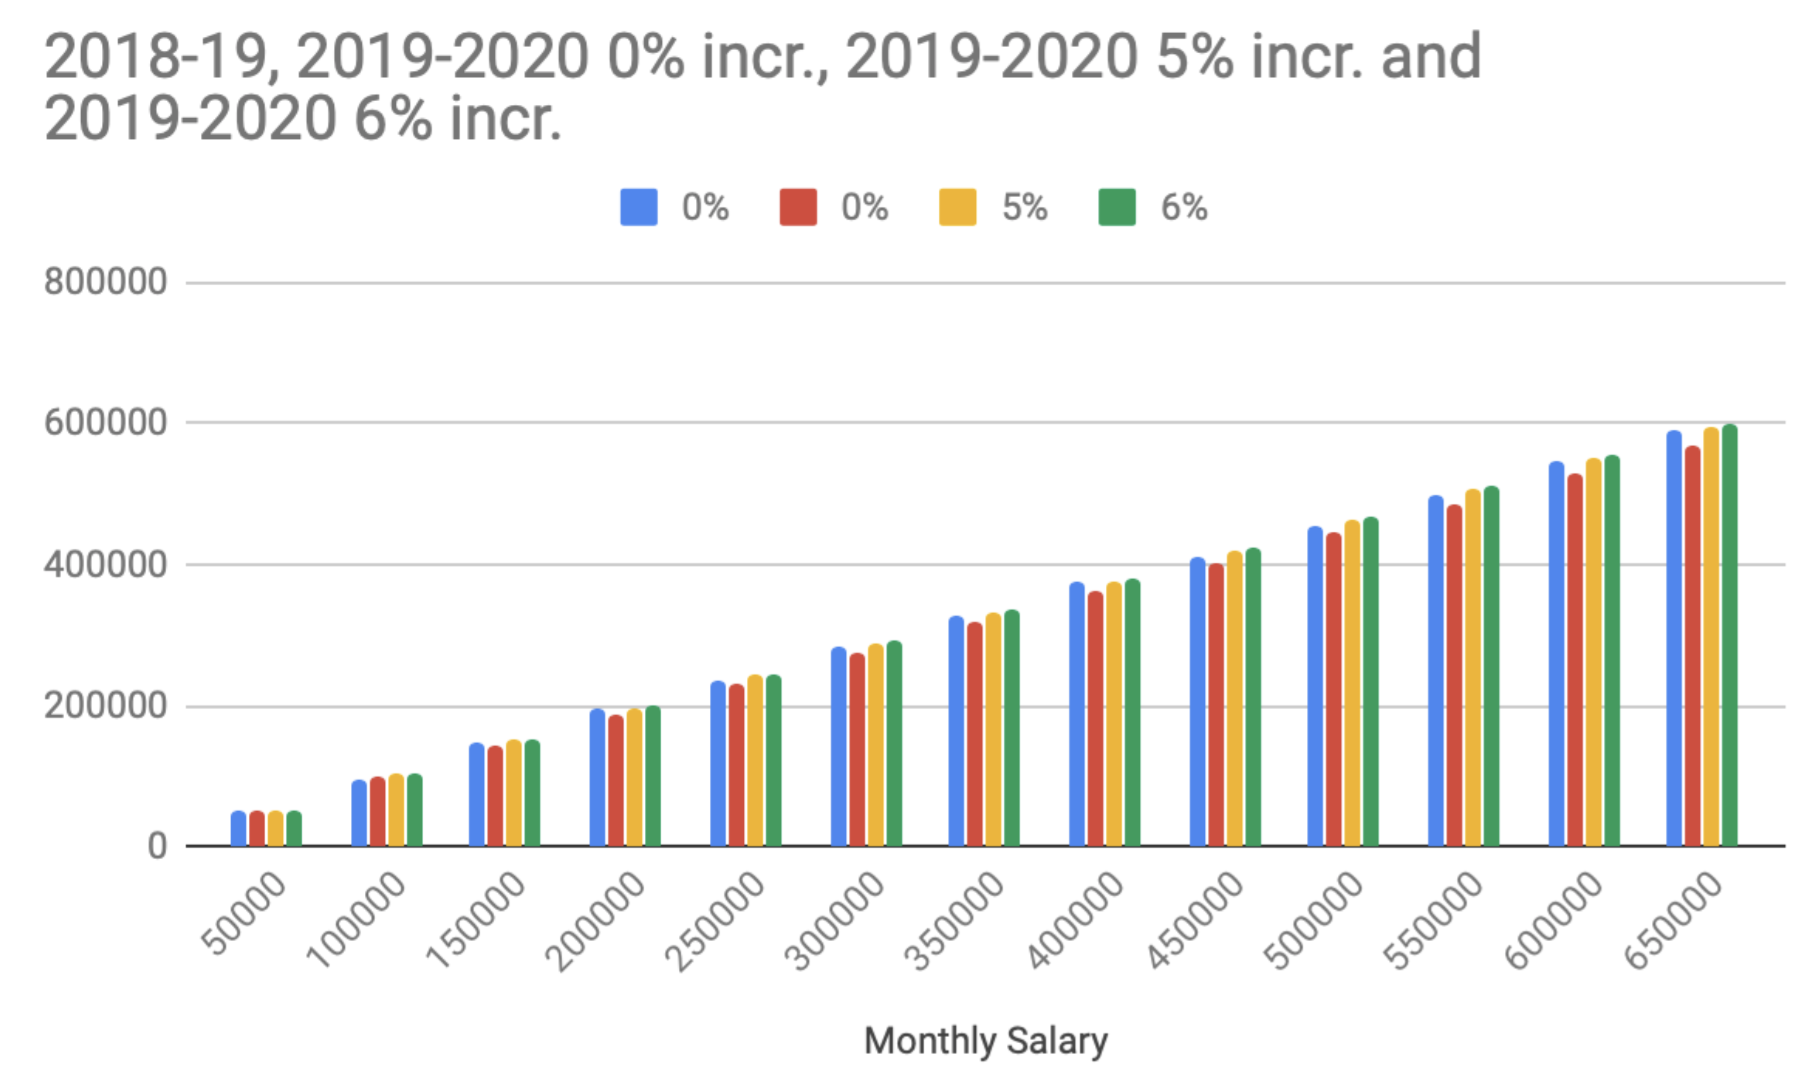
\includegraphics[scale=.2]{salary_chart.png}
	\caption{Comparisons of Take Home Salaries with new Tax Scheme with 0\%, 5\%, and 6\% Increments}
	\label{fig:comp-salary}
\end{figure}
	
\end{document}